% Sample LaTeX file for creating a paper in the Morgan Kaufmannn two
% column, 8 1/2 by 11 inch proceedings format.

\documentclass[11pt]{article}
%\usepackage{proceed2e}
\usepackage[margin=.75in]{geometry}

% Set the typeface to Times Roman
\usepackage{times}

\usepackage{microtype}
\usepackage{graphicx}
%\usepackage{subfigure}
\usepackage{booktabs} % for professional tables
\usepackage{amssymb,amsmath,amstext,amsgen,amsfonts,amsthm,mathrsfs}
\usepackage{relsize}
\usepackage{multicol, blindtext}
%\usepackage{caption}
\usepackage{subcaption}
\usepackage{multirow}
\usepackage[table]{xcolor}
\usepackage{mwe}
\usepackage{tikz}
\usepackage{algorithm}
\usepackage{algorithmic}
\usepackage[round]{natbib}
\setlength{\bibsep}{0.0pt}
\bibliographystyle{abbrvnat}
\usepackage{enumitem}
\usepackage{float}
\usepackage{bm}

\makeatletter
\renewcommand\@biblabel[1]{}
\renewenvironment{thebibliography}[1]
     {\section*{\refname}%
      \@mkboth{\MakeUppercase\refname}{\MakeUppercase\refname}%
      \list{}%
           {\leftmargin0pt
            \@openbib@code
            \usecounter{enumiv}}%
      \sloppy
      \clubpenalty4000
      \@clubpenalty \clubpenalty
      \widowpenalty4000%
      \sfcode`\.\@m}
     {\def\@noitemerr
       {\@latex@warning{Empty `thebibliography' environment}}%
      \endlist}
\makeatother
\newlength{\bibitemsep}\setlength{\bibitemsep}{.25\baselineskip plus .03\baselineskip minus .05\baselineskip}
\newlength{\bibparskip}\setlength{\bibparskip}{0pt}
\let\oldthebibliography\thebibliography
\renewcommand\thebibliography[1]{%
  \oldthebibliography{#1}%
  \setlength{\parskip}{\bibitemsep}%
  \setlength{\itemsep}{\bibparskip}}


%\usepackage{adjustbox}
\usepackage{array}

\pagestyle{empty}

\newcommand{\bracedincludegraphics}[2][]{%
  \sbox0{$\vcenter{\hbox{\includegraphics[#1]{#2}}}$}%
  \left\lbrace
    \vphantom{\copy0}
  \right.\kern-\nulldelimiterspace
  \underbrace{\box0}}

\usepackage{booktabs, makecell, tabularx}
\usepackage{rotating}
\usepackage[export]{adjustbox}

% Measure the image height
\newsavebox\mybox
\savebox\mybox{%
  \begin{minipage}[t]{0.1\linewidth}
    \includegraphics[width=0.5\linewidth]{example-image-a}
  \end{minipage}%
}

\newtheorem{theorem}{Theorem}[section]
\newtheorem{proposition}[theorem]{Proposition}
\newtheorem{lemma}[theorem]{Lemma}

\theoremstyle{remark}
\newtheorem{remark}[theorem]{Remark}
\newtheorem{conj}{Conjecture}

\theoremstyle{definition}
\newtheorem{definition}{Definition}[section]



\title{Data Science II Project: Travelers Competition}

\author{Aaron Palmer} % LEAVE BLANK FOR ORIGINAL SUBMISSION.
          % UAI  reviewing is double-blind.

% The author names and affiliations should appear only in the accepted paper.
%
%\author{ {\bf Harry Q.~Bovik\thanks{Footnote for author to give an
%alternate address.}} \\
%Computer Science Dept. \\
%Cranberry University\\
%Pittsburgh, PA 15213 \\
%\And
%{\bf Coauthor}  \\
%Affiliation          \\
%Address \\
%\And
%{\bf Coauthor}   \\
%Affiliation \\
%Address    \\
%(if needed)\\
%}

\begin{document}

\maketitle

\section{Abstract}
The Travelers data challenge is a competition seeking the highest AUC when predicting the binary outcome of policy cancellation. The large data size, over 1 million rows in training and half a million testing set, necessitates a pragmatic approach to modeling by making use of parallel and distributed modeling methods. Multiple imputation is used to impute missing values, a basic but principled feature exploration and engineering is conducted, along with utilizing several machine learning models, that fall under the class of ensembling methods, are used to `stack' predictions. 
\section{Introduction: Problem Definition}
The challenge here is to use historical policy data to create a retention model to predict policies most likely to cancel at the end of the current term. While the problem is primarily concerned with predictive performance, understanding which variables are influential in causing policy cancellation is important. 

The two measures for performance are area under the curve (AUC) and quality of code; though actionable business insight is encouraged. The Nutmeg data set is based on 4 years of property insurance policies from 2013 to 2017. There are roughly 1 million policies in the training data set, with each policy having a single observation. There are almost 250,000 policies that were canceled during the effective term.

For this project, a number of interesting modeling challenges are brought up. Each section will discuss the modeling issue at hand, and provide a solution.  As the data is simulated, it becomes inappropriate to use our own experience and intuition when looking at features and how they might interact. Hence an objective, methodological approach needs to be taken. Section 3 will discuss variable characteristics. Section 4 deals with missing data, with section 5 covering data exploration and feature engineering. In section 6 we discuss the models used, and section 7 details how model aggregation from multiple imputation might be accomplished. We conclude with section 8 where we discuss room for improvement to be explored in future work.
\section{Variables}\label{subsec:vars}
Variables in the data set are listed in Table (\ref{tab:var_tab}) along with a brief description and the associated data type. 
\begin{table}[]
\caption{Variables included in training and testing set along with description, variable type, and missing counts.}
\scalebox{.8}{
\begin{tabular}{|l|l|l|l|l|}
\hline
Variable            & Description & Variable Type & Train Miss & Test Miss            \\ \hline
id                  & Policy id (cannot be used in model) & unique policy identifier & 0        & 0 \\ \hline
claim               & Occurrence of claim (0=no, 1=yes) & categorical: nominal (2 levels) & 986      & 427     \\ \hline
gender              & Gender of policyholder & categorical: nominal (2 levels) & 960      & 372     \\ \hline
marital status      & Marital status of policyholder (0=no, 1=yes) & categorical: nominal (2 levels) & 994      & 431     \\ \hline
coverage type       & Type of coverage & categorical: nominal (3 levels) & 980      & 405     \\ \hline
sales channel       & Medium through which policy was purchased & categorical: nominal (3 levels) & 1025     & 394    \\ \hline
dwelling type       & Type of dwelling & categorical: nominal (4 levels) & 993      & 422    \\ \hline
house color         & Color of house & categorical: nominal (4 levels) & 945      & 406    \\ \hline
zipcode     & Zip code of the property  & categorical: nominal (310 levels) & 951      & 370   \\ \hline
cancel				& cancellation indicator (0=no, 1=yes). Response variable. & categorical: nominal (2 levels) & 0 & NA \\ \hline
credit              & Financial credit level of policyholder & categorical: ordinal (3 levels) & 907      & 380   \\ \hline
year                & Year of the policy & positive integer & 0        & 0         \\ \hline
tenure              & Number of years with Kangaroo & positive integer & 980      & 401         \\ \hline
length at residence & Length at residence (how long policyholder lived at property) & positive integer & 967      & 380         \\ \hline
number of adults    & Number of adults in the property & positive integer & 931      & 405         \\ \hline
number of children  & Number of children in the property & positive integer & 938      & 398         \\ \hline
age of policyholder & Age of policyholder & positive integer & 1002     & 391         \\ \hline
premium             & Price of the policy & positive real & 957      & 387            \\ \hline
\end{tabular}}\label{tab:var_tab}
\end{table}
Prior to any real data exploration, quick overview of the data yields many issues that will need to be addressed. Under the variable `dwelling type' there exists a category ``Landlord" that is in the testing set, and is not present in the training set. The training data only contains years 2013 - 2016 while the testing set is only 2017. In the training set there are errors in the response variable; $3,452$ rows have an incorrect value of $-1$ which is outside the allowable set of $\{0,1\}$. The training set contains 1,048,575 observations, and within this 14,410 rows contain at least one missing variable. This represents 1.37\% corruption rate. The test set contains 444,430 observations also with a 1.37\% corruption rate. Missing counts by variable for the training and testing set can be seen in the last two columns of Table (\ref{tab:var_tab}). The data contains unbalanced class sizes $\{0: 792,026, 1: 253,097 \}$. Other than year and dwelling type, it would be of interest to determine whether or not the training and testing sets possess similar distributions (otherwise modeling would be a challenge).

Prior to any imputation, a new variable `state' was created based on the `zipcode' variable. Using a factor that has 310 levels is not feasible, and so either it needed to be converted into a continuous variable via latitude and longitude, or be substantially reduced. Modeling with latitude and longitude did not improve performance, however collapsing zipcode to state lead to a roughly 6\% increase in AUC. There were only 6 states in the data set after converting zipcode: Arizona, Colorado, Iowa, Pennsylvania, Virginia, and Washington.
\section{Imputing Missing values}
Many statistical and machine learning models require complete data. If missing data is present, poor methods to address this may do more harm than good. With a fairly low corruption rate on the training set, one possible solution could be simply removing these rows before modeling. However, simply removing rows may result in a loss of, potentially valuable, information. More importantly, as the test set contains missing values the predictive algorithm needs to make predictions (unless of course the predictive algorithm can tolerate missing data). There exist a variety of techniques to deal with missing data. One way is through imputation.

There are multiple ways to conduct imputation, several of which have ready made packages in R and Python. We briefly recap the concepts of missingness. First, missing completely at random (MCAR) dictates that the tendency of a data point to be missing has no relationship between any other observed or unobserved variables. Using only complete cases is valid here. This is a very strong condition to satisfy, and in practice there is no way to verify it. Slightly weaker is missing at random (MAR). Many methods assume MAR (for the Travelers data challenge this is what we will assume). MAR dictates that the propensity of a data point to be missing is \textit{only} related to some of the observed data. This assumption is not statistically verifiable, and so its use should be justified. Finally, missing not at random (MNAR) denotes the missing value is related to the reason it is missing. 

The simplest method(s), called generalized imputation (GI), for continuous variables with missing values use the mean or median values computed from the non-missing data, while for categorical data the mode could be used. A slightly more advanced method to GI would be similar case imputation (SCI). Here a subgroup is used for computation. An example would be using females to impute missing female data and Males to impute missing male data. One of the more common methods is called multiple imputation. The general idea follows 3 steps:
\begin{enumerate}[nolistsep]
	\item Impute missing values with values drawn from some distributions to generate $m$ complete cases data sets.
	\item Perform the same analysis on each of the $m$ data sets.
	\item Pool the results in some fashion.
\end{enumerate}
The MICE package \citep{buuren2010}, short for multivariate imputation via chained equations, is an R implementation for performing multiple imputation. The methods covered by this package can handle imputing a variety of data types. For continuous variables predictive mean matching (PMM) can be used. For binary variables logistic regression is used. For nominal categorical variables, Bayesian polytomous regression is used, while for ordinal categorical variables a proportional odds model is used for imputation. All of these data types are present in the Travelers data challenge. Unfortunately, MICE doesn't automatically detect data types, and so each variable data type will need to be set up manually. 

As this is a data competition, we cannot simply omit predictions for certain rows. Therefore, missing data on the test set must also be imputed in some manner. Since the distribution of train and test set seemed to be similar, we decided to impute on the combined test and train set using all variables except `cancel' and `id.' One of the issues present in imputing missing values is scalability. With large samples, it can take a long time to run, though it is possible to parallelize each of the $m$ sets. Due to resource limitations and data size when using the UCOnn HPC, maximum iterations was set to $5$ and number of imputed sets $m = 3$.

Several version of imputation were tried. Any outliers in the data, for example in `age' were set to missing and imputed. Dwelling type `Landlord' in the testing set was set to missing and imputed in one version, and in another it was set to `House.' Neither version was distinctly better than the other, though this may have been a result of the limited imputing time.
\section{Data Exploration}
As the number of variables is manageable, we can use scatter plots and histograms to visually see if there are any standout relationships we can make use of in the model. With such large data size, the scatter plot can only use a sub-sample (which we used 10,000).
\begin{figure}[H]
    \centering
    \begin{minipage}{.5\linewidth}
        \centering
        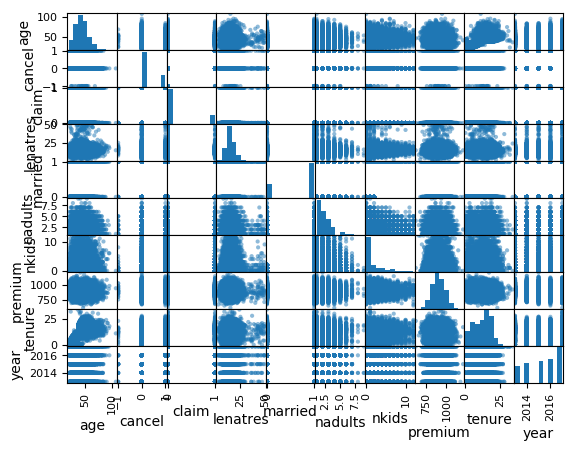
\includegraphics[width=\linewidth]{scatter2.png}
        \caption{Two-way scatter plot of covariates}
        \label{fig:scatter}
    \end{minipage}%
    \begin{minipage}{0.5\linewidth}
        \centering
        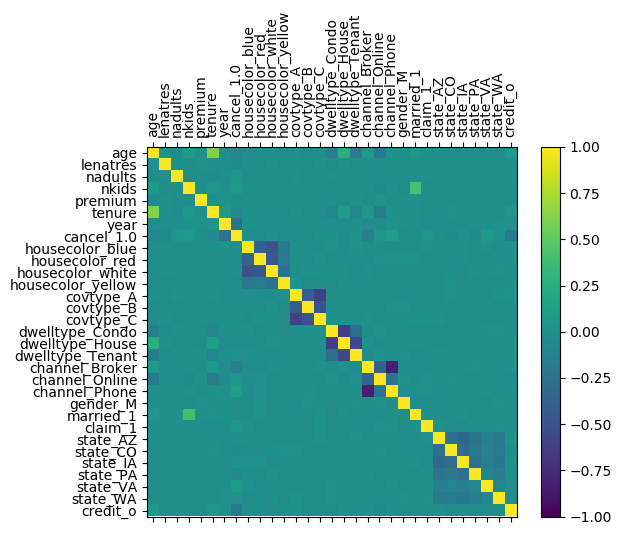
\includegraphics[width=\linewidth]{corr2.png}
        \caption{Correlation heatmap after categorical variables have been dummied.}
        \label{fig:corr}
    \end{minipage}
\end{figure}
If we look at the top absolute correlations between features that aren't in the same category, we can see that $age$ vs $tenure$ has a correlation of $0.610990$, $nkids$ vs $married$  has a correlation of $0.405856$, and $age$ vs $dwelltype\_House$ has a correlation of $0.263813$. These are candidates to consider adding into the model. Another criteria worth exploring is maximal information coefficient \citep{reshef2011} which is a measure of the strength of the linear or \textit{non-linear} association between two variables. Unfortunately, a pythonic version for windows wasn't immediately available, so we kept with simple correlation.
\subsection{Data Pre-processing, Normalization \& Standardization}
Depending on the method chosen for modeling policy cancellation, normalization or standardization may be necessary. When data is normalized it re-scales the data into the range $[0,1]$, while data standardization brings the data to have mean zero and standard deviation 1. For example, it is preferable to use standardization when training support vector machines. It is not necessary to standardize or scale data prior to fitting methods based on trees. 

For XGBoost, neural networks and many other models to run correctly, it can only take numeric data. Therefore, all categorical variables needed to be dummied prior to model fitting. For example, if the current variable is $coverage\_type$ taking values from the set $\{A, B, C\}$ then if $coverage\_type = A$ then this is represented by $[1,0,0]$, and if $B$ it is $[0,1,0]$. The continuous or integer valued data can remain untouched. Interestingly, there are a few ways to encode ordinal data. It can either be coded as $0,1,2$ etc, however this implicitly assumes each level is equally spaced away. Another way may be to encode categorical using the proportions of its categories. This was tried, but didn't make much difference.
\section{Methods}
The major consideration for all models used will be their ability to scale. The two primary methods will be using classification and regression trees (CART) at scale (with boosting (GBM)), and using recent advances in the field of deep learning to train neural networks. Each model has advantages for training at scale and have been shown to empirically work very well on a variety of tasks. For example tree based methods have an ability to determine variable importance while neural networks are extremely powerful function approximators reaching state-of-the-art accuracy on prediction problems. Unfortunately, neural nets are still rather limited when understanding how variables influence the model. The goal for modeling will be to create an ensemble of tree based and neural network models, leveraging the benefits of each as best as possible across each of the $m=3$ imputed data sets. When making predictions on the test set, there were three options. One is to set $year=2017$ to $year=2016$ under the assumption that the best prediction of tomorrow is today, another is to simply not use $year$ in modeling, or finally assume forecasting one year ahead is reasonable. For this project, we set all testing years to be $2016$.
\subsection{XGBoost}
XGBoost \citep{chen2016}, which stands for Extreme Gradient Boosting, is a highly scalable ensemble learning method that handles large data very well. For a given data set with $n$ examples and $m$ features, a tree ensemble models uses $K$ additive functions to predict the output $\hat{y}_i = \phi(\mathbf{x}_i) = \sum\limits_{k=1}^{K} f_k(\mathbf{x}_i), \quad f_k \in \mathcal{F}$, where $\mathcal{F} = \{f(\mathbf{x} = w_{q(\mathbf{x})}\}(q: \mathbb{R}^{m} \rightarrow T, w \in \mathbb{R}^{T})$ is the space of regression trees. $q$ represents the structure of each tree mapping an example to the corresponding leaf index, $T$ is number of leaves in tree. Each $f_k$ is an independent tree structure $q$ with leaf weights $w$. The goal is to minimize the regularized objective $\mathcal{L}(\phi) = \sum\limits_{i} \ell(\hat{y}_i, y_i) + \sum\limits_{k} \Omega(f_k)$ where $\Omega(f) = \gamma T + \frac{1}{2} \lambda ||w||^2$, where $\ell$ is a differentiable convex loss function and $\Omega$ penalizes model complexity. For gradient boosting, a new objective $\mathcal{L}^{(t)} = \sum\limits_{i=1}^n \ell(y_i, \hat{y}_i^{(t-1)} + f_t(\mathbf{x}_i)) + \Omega(f_t)$ where $\hat{y}_i^{(t-1)}$ is the prediction of instance $i$ at the $t^{th}$ iteration. We want to add a new $f_t$ such that the objective is minimized.

There are a number of hyper-parameters that need to be tuned. Importantly, XGBoost is able to handle unbalanced classes by scaling the positive weights. This was set to $\frac{\sum_{y_i \in \mathbf{y}} 1_{\{y_i = 0\}}}{\sum_{y_i \in \mathbf{y}} 1_{\{y_i = 1\}}}$ which was about $3$. Both cross-validation with grid search and randomized searching with cross-validation were used but this ended up being very expensive to run. Using a combination of these and manual turning, we arrived at a maximum tree depth of 8, and a learning rate $\eta=0.02$. To help prevent over-fitting we can sub-sample from the training instances prior to growing trees. Here we found that using $0.7$ worked well. The number of estimators was set to $500$. Similar parameters were used for each of the imputation sets. Another method for parameter tuning, to be explored in the future, is Bayesian optimization \citep{snoek2012}. 

After training XGBoost on each of the imputed data sets using different seeds, we can see how it performs on each models' hold-out set in Fig.(\ref{fig:auc}). To get an idea of the relative importance of the features XGBoost allows a visualization of the number of times a particular feature was split on. This can be seen in Fig.(\ref{fig:imp_feats}). Premium, age and length at the residence are not particularly surprising (assuming real data reflects the same patterns), but two the interaction variables created earlier, $age \times tenure$, $age \times dwelltype\_House$, were high up on the list. Interestingly, $nkids \times married$ wasn't so high.
\begin{figure}[H]
    \centering
    \begin{minipage}{.5\linewidth}
        \centering
        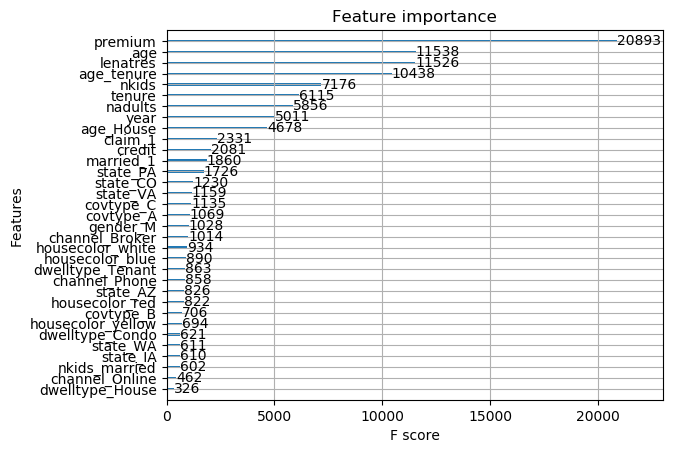
\includegraphics[width=\linewidth]{imp_feats.png}
        \caption{Feature Importance}
        \label{fig:imp_feats}
    \end{minipage}%
    \begin{minipage}{0.5\linewidth}
        \centering
        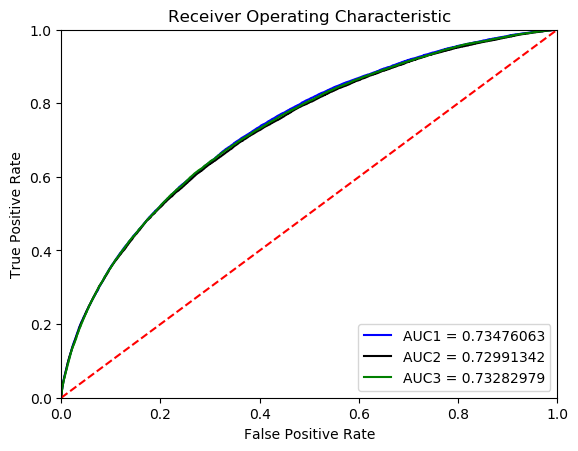
\includegraphics[width=\linewidth]{auc2_XGBoost.png}
        \caption{Hold-out set AUC}
        \label{fig:auc}
    \end{minipage}
\end{figure}
\subsection{Neural Networks}
Neural networks \citep{goodfellow2016} are powerful black-box function approximators capable of capturing complex relationships within data. From computer vision to natural language processing, they have produced state-of-the-art results on a variety of tasks. However, when applying them to business type problems where data do not possess the properties that allow convolutional neural networks to work well, like spatio-temporal relationships, training the models can become a challenge. If given too much capacity for the task at hand, they become prone to over-fitting. 

However, even with their drawbacks neural nets are capable of modeling very large datasetse by using small batches of data combined with stochastic gradient descent. Unfortunately with very large data, training can take a while and due to the highly nonlinear loss surface it is difficult to tell whether optimization has slowed or a local minima has trapped progress. Nevertheless, we used TensorFlow \citep{abadi2016} to fit a multi-layer network. The architecture consisted of two hidden layers, the first contained 20 nodes and the second one contained 10. A rectified linear unit activation function was used to help with vanishing gradients. RMSProp was used as an optimizer, with an initial learning rate of $1\times 10^{-5}$ with a batch size of 500. After reaching around $71.8\%$ AUC, learning became very difficult. Changing learning rates resulted in the same issue, so careful tuning is necessary here. Training was much slower than XGBoost, even with GPU support. Therefore we spent our time tuning a single model. The final AUC can be seen in Fig.(\ref{fig:net_auc}).
\begin{figure}[]
    \centering
    \begin{minipage}{.5\linewidth}
        \centering
        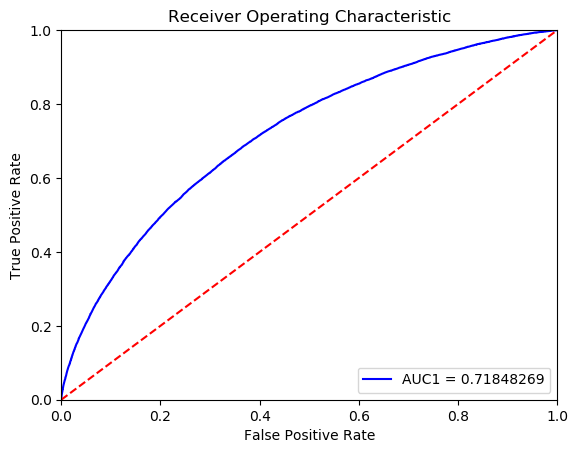
\includegraphics[width=\linewidth]{auc2_network.png}
        \caption{Neural Net as classifier AUC on hold-out set}
        \label{fig:net_auc}
    \end{minipage}%
    \begin{minipage}{0.5\linewidth}
        \centering
        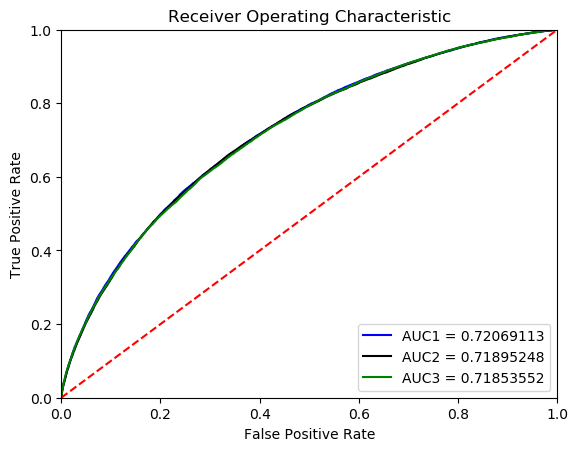
\includegraphics[width=\linewidth]{auc2_logistic.png}
        \caption{Logistic Regression Hold-out AUC: all sets}
        \label{fig:auc_logit}
    \end{minipage}
\end{figure}
\subsection{Logistic Regression}
For pure interpretability logistic regression was modeled on each of the imputed sets. The hold out AUC can be seen in Fig.(\ref{fig:auc_logit}). The striking part here is that a model as simple as logistic regression was not \textit{too} much worse than some of the more complex models. If one is willing to sacrifice a percent or so of AUC, then the model can be interpreted better than either XGBoost or the neural network. For example, the odds of canceling the policy increase by about 8.34\% with each additional adult on the policy. As far as actionable business recommendations, this method offers better insight.
\section{Model Ensembling}
While training the tree algorithms and neural networks can be challenging in themselves, figuring out a way to combine the outputs will be a whole new challenge. One possible method is to use the predictions from each base model as features for another model. Using the true $y_i$ as the response, and predictions from each model as new feature inputs, a new model can be trained. This is often referred to as `model stacking,' and even simple models like logistic regression have benefits when put together in this framework. This kind of hierarchical model can often perform well as the second level learner can discover which instances are better predicted by which model. This model offers a kind of `weighting' function instead of naively averaging predictions. Unfortunately, this method traditionally works off models built using a \textit{single} data set. Utilizing this approach with \textit{multiple} imputed data sets makes things more challenging as multiple models will be built on multiple data sets, and predictions will be done on multiple test sets. For our tasks, and due to time constraints placed on the training algorithms we opted for a naive approach of simply averaging the predicted probabilities from each model via $\hat{y}_i = \frac{1}{J} \sum\limits_{j=1}^{J} \hat{y}_{j, i}$ where $\hat{y}_{j, i}$ is the $j^{th}$ model for subject $i$. These final prediction probabilities can be used for submission to Kaggle.
\section{Challenges and Future Work (Interesting Directions to Explore)}
There were a number of obstacles present in this data challenge. First and foremost was the restriction on imputation. Cutting imputation time short very likely hindered the models, though hold-out sets did see performance improvement even with the 5 iterations done. Hyper-parameter tuning was certainly a challenge, and Bayesian optimization will be explored in the future (I'm interested in this). Finally, while XGBoost can output feature importance, it doesn't give much insight as to how a business policy might be constructed to influence retention, i.e. age is important but doesn't tell us if old or young are more likely to cancel. However, a simpler model like multiple logistic regression can tell us that the odds of canceling decrease by 2.69\% with each additional year of customer age. One solution for interpreting more complex models might be Shapley values \citep{lundberg2017}. This is absolutely something we will explore as it has the ability to offer insight into black-box models. Hopefully, Kaggle will allow model submissions past the deadline.
\newpage
\bibliography{biblio}
\end{document}
